\PassOptionsToPackage{unicode}{hyperref}
\PassOptionsToPackage{naturalnames}{hyperref}

\documentclass[xcolor=dvipsnames, aspectratio=149, 12pt]{beamer}


\usepackage{etex}
%\usetheme{Darmstadt}
\usetheme{Madrid}
%\usecolortheme[named=NavyBlue]{structure}
\usecolortheme{whale}

%\usetheme{Frankfurt}  %\usecolortheme{default}

%\useoutertheme{infolines}

\mode<presentation>

\setbeamersize{text margin left=5mm}
\setbeamersize{text margin right=5mm}
\setbeamertemplate{footline}[page number]{}
\setbeamertemplate{blocks}[rounded][shadow=false]
\setbeamertemplate{title page}[default][colsep=-4bp,rounded=true]
\beamertemplatenavigationsymbolsempty
    %\setbeamertemplate{footline}{%
     % \raisebox{5pt}{\makebox[\paperwidth]{\hfill\makebox[10pt]{\scriptsize\insertframenumber}}}}
      
\addtobeamertemplate{block begin}{\setlength{\textwidth}{0.99\textwidth}}{}
\addtobeamertemplate{block begin}{\setlength\abovedisplayskip{0pt}}
%\addtobeamertemplate{block begin}{\vspace{-25pt}}{}


\usepackage{ucs}
\usepackage[utf8x]{inputenc}
\usepackage[greek,english]{babel}
\newcommand{\en}{\selectlanguage{english}}
\newcommand{\el}{\selectlanguage{greek}}
\usepackage[T1]{fontenc}
\usepackage{lmodern}

\usepackage[absolute,overlay]{textpos}

\newcommand{\sq}{\selectlanguage{english}\color{red!70!blue}\bf}
\newcommand{\bb}{\selectlanguage{greek}\color{blue!50!black}\bf}
\newcommand{\ra}{\selectlanguage{english}\color{blue!90!red}\em\large}
\newcommand{\enb}{\selectlanguage{english}\color{blue}}
\newcommand{\ex}[1]{\begin{math}\partial{#1}\end{math}}

\newcommand{\cgg}{\selectlanguage{english}\color{green!60!black}\bf}
\newcommand{\cmm}{\selectlanguage{english}\color{red!50!blue}\bf}

\newcommand{\cee}{\selectlanguage{greek}\color{red!90!blue}\bf\large}
\newcommand{\bbl}{\color{blue!90!black}\bf}
\newcommand{\crr}{\color{red!90!blue}\bf}
\newcommand{\cbb}{\color{blue!90!black}\bf}

\colorlet{colBC}{Apricot!50}

%\usepackage{enumitem}
\usepackage{booktabs}
\usepackage{hyperref}
\usepackage{listings}
\usepackage{fancyvrb}
\usepackage{listings}
\usepackage{amsmath}
\usepackage{amssymb}
\usepackage{mathtools}
\usepackage{mathrsfs}
\usepackage{colortbl}
\usepackage{graphicx}
\usepackage{chngcntr}
%\usepackage{subfig}
%\usepackage{subcaption}}
\usepackage{pgf, tikz}
\usepackage{pgfplots} %\pgfplotsset{compat=newest}
\usepackage{pgfplotstable}
\usepackage{comment}
\usepackage[normalem]{ulem}

\usepackage[tikz]{bclogo}
\usetikzlibrary{matrix}
\usetikzlibrary{arrows,automata,shapes,calc,positioning,fit}
\usetikzlibrary{backgrounds,shadows,trees}


\usetikzlibrary{calc}
%\usepackage{booktabs}
\usepackage{attachfile}

\definecolor{blue10}{RGB}{135, 204, 255}
\definecolor{blue90}{RGB}{0, 0, 204}


\DefineVerbatimEnvironment{codeE}{Verbatim}
{
  frame            = leftline,
  samepage         = true,
  commandchars     = &\{\}, 
  rulecolor=\color{black!50!white}, framerule=3px,
  baselinestretch  = 1,
  fontsize         = \small
}

\DefineVerbatimEnvironment{codeR}{Verbatim}
{
  frame            = leftline,
  samepage         = true,
  numbers          = left,
  numbersep        = 6pt,
  commandchars     = &\{\}, 
  rulecolor=\color{red!90!black}, framerule=3px,
  baselinestretch  = 1,
  fontsize         = \small
}

\DefineVerbatimEnvironment{codeM}{Verbatim}
{
  frame=leftline,  framerule=2px,  rulecolor=\color{blue},
  samepage=true, numbers=left,   numbersep=6pt,
  commandchars=&\{\}, baselinestretch=1, fontsize=\small
}

\DefineVerbatimEnvironment{codeO}{Verbatim}
{
  frame=leftline,  framerule=2px,  rulecolor=\color{blue},
  samepage=true, numbers=left,   numbersep=6pt,
  commandchars=&\{\}, baselinestretch=1, fontsize=\small
}

\DefineVerbatimEnvironment{SQL}{Verbatim}
{
  frame=leftline,  framerule=2px,  rulecolor=\color{blue},
  samepage=true, numbers=left,   numbersep=6pt,
  commandchars=&\{\}, baselinestretch=1, fontsize=\small
}

\DefineVerbatimEnvironment{codeC}{Verbatim}
{
  frame=leftline,  framerule=2px,  rulecolor=\color{blue},
  samepage=true, numbers=left,   numbersep=6pt,
  commandchars=&\{\}, baselinestretch=1, fontsize=\small
}


\newcommand{\code}[1]{\en \textsl{#1}}{\el}
\newcommand{\ojoinaux}{\setbox0=\hbox{$\bowtie$}%
  \rule[-.02ex]{.25em}{.4pt}\llap{\rule[\ht0]{.25em}{.4pt}}}
\newcommand{\ojoin}{\mathbin{\ojoinaux\mkern-5.6mu\bowtie\mkern-5.7mu\ojoinaux}}
\newcommand{\lojoin}{\mathbin{\ojoinaux\mkern-5.6mu\bowtie}}
\newcommand{\rojoin}{\mathbin{\bowtie\mkern-5.7mu\ojoinaux}}

\newcommand{\stirlingtwo}[2]{\genfrac{\lbrace}{\rbrace}{0pt}{}{#1}{#2}}

\logo{
\includegraphics[width=2.5cm,height=2.5cm,keepaspectratio]{../common/SQL2.jpg}}

\AtBeginSection[]
{ \el
  \begin{frame}<beamer>
    \frametitle{Περιεχόμενα}
    \begin{minipage}{\wE}
      \tableofcontents[currentsection]
    \end{minipage} 
  \end{frame}
}

\AtBeginSubsection[]
{
  \begin{frame}<beamer>
    \frametitle{Περιεχόμενα}
    \begin{minipage}{\wE}
      \tableofcontents[currentsubsection]
    \end{minipage}   
  \end{frame}
}


\newcommand{\wE}{0.88\textwidth}
\newcommand{\wN}{0.92\textwidth}



\newcommand{\men}[1] {\selectlanguage{english}#1\selectlanguage{greek}}
\newcommand{\mene}[1] {\selectlanguage{english}\emph{#1}\selectlanguage{greek}}
\newcommand{\mgr}[1] {\selectlanguage{greek}#1\selectlanguage{english}}
\newcommand{\mgre}[1] {\selectlanguage{greek}\emph{#1}\selectlanguage{english}}


% η \tsql τυπώνει SQL
\newcommand{\tsql}{\selectlanguage{english}SQL\selectlanguage{greek}}
\newcommand{\tasql}{\selectlanguage{english}ANSI-SQL\selectlanguage{greek}}
\newcommand{\tddl}{\selectlanguage{english}DDL\selectlanguage{greek}}
\newcommand{\tdml}{\selectlanguage{english}DML\selectlanguage{greek}}

\newcommand{\tselect}{\selectlanguage{english}SELECT\selectlanguage{greek}}
\newcommand{\tselectd}{\selectlanguage{english} SELECT$\ldots$ \selectlanguage{greek}}
\newcommand{\tfrom}{\selectlanguage{english}FROM\selectlanguage{greek}}
\newcommand{\tfromd}{\selectlanguage{english} FROM$\ldots$ \selectlanguage{greek}}
\newcommand{\twhere}{\selectlanguage{english}WHERE\selectlanguage{greek}}
\newcommand{\twhered}{\selectlanguage{english} WHERE $\ldots$\selectlanguage{greek}}
\newcommand{\torderby}{\selectlanguage{english}ORDER BY\selectlanguage{greek}}
\newcommand{\tgroupby}{\selectlanguage{english}GROUP BY\selectlanguage{greek}}
\newcommand{\thaving}{\selectlanguage{english}HAVING\selectlanguage{greek}}
\newcommand{\trollup}{\selectlanguage{english}ROLLUP\selectlanguage{greek}}
\newcommand{\tnull}{\selectlanguage{english}NULL\selectlanguage{greek}}
\newcommand{\tunk}{\selectlanguage{english}UNK\selectlanguage{greek}}
\newcommand{\tnotnull}{\selectlanguage{english}NOT NULL\selectlanguage{greek}}
\newcommand{\ttrue}{\selectlanguage{english}TRUE\selectlanguage{greek}}
\newcommand{\tfalse}{\selectlanguage{english}FALSE\selectlanguage{greek}}
\newcommand{\tlike}{\selectlanguage{english}LIKE\selectlanguage{greek}}
\newcommand{\tand}{\selectlanguage{english}AND\selectlanguage{greek}}
\newcommand{\tor}{\selectlanguage{english}OR\selectlanguage{greek}}
\newcommand{\tnot}{\selectlanguage{english}NOT\selectlanguage{greek}}
\newcommand{\tdistinct}{\selectlanguage{english}DISTINCT\selectlanguage{greek}}
\newcommand{\tavg}{\selectlanguage{english}AVG()\selectlanguage{greek}}
\newcommand{\tsum}{\selectlanguage{english}SUM()\selectlanguage{greek}}
\newcommand{\tmin}{\selectlanguage{english}MIN()\selectlanguage{greek}}
\newcommand{\tmax}{\selectlanguage{english}MAX()\selectlanguage{greek}}
\newcommand{\tcount}{\selectlanguage{english}COUNT()\selectlanguage{greek}}
\newcommand{\tcounta}{\selectlanguage{english}COUNT(*)\selectlanguage{greek}}
\newcommand{\tall}{\selectlanguage{english}ALL\selectlanguage{greek}}
\newcommand{\tany}{\selectlanguage{english}ANY\selectlanguage{greek}}
\newcommand{\texists}{\selectlanguage{english}EXISTS\selectlanguage{greek}}
\newcommand{\tdefault}{\selectlanguage{english}DEFAULT\selectlanguage{greek}}
\newcommand{\tconstraint}{\selectlanguage{english}CONSTRAINT\selectlanguage{greek}}
\newcommand{\tondelcas}{\selectlanguage{english}ON DELETE CASCADE\selectlanguage{greek}}
\newcommand{\tonupcas}{\selectlanguage{english}ON UPDATE CASCADE\selectlanguage{greek}}

\newcommand{\tjoin}{\selectlanguage{english}JOIN\selectlanguage{greek}}

\newcommand{\tinsert}{\selectlanguage{english}INSERT\selectlanguage{greek}}
\newcommand{\tdelete}{\selectlanguage{english}DELETE\selectlanguage{greek}}
\newcommand{\tupdate}{\selectlanguage{english}UPDATE\selectlanguage{greek}}

\newcommand{\tcreatedb}{\selectlanguage{english}CREATE DATABASE\selectlanguage{greek}}
\newcommand{\tcreatetab}{\selectlanguage{english}CREATE TABLE\selectlanguage{greek}}
\newcommand{\taltertab}{\selectlanguage{english}ALTER TABLE\selectlanguage{greek}}
\newcommand{\tprikey}{\selectlanguage{english}PRIMARY KEY\selectlanguage{greek}}
\newcommand{\tforkey}{\selectlanguage{english}FOREIGN KEY\selectlanguage{greek}}
\newcommand{\tdropt}{\selectlanguage{english}DROP TABLE\selectlanguage{greek}}
\newcommand{\tdropv}{\selectlanguage{english}DROP VIEW\selectlanguage{greek}}

\newcommand{\tgrant}{\selectlanguage{english}GRANT\selectlanguage{greek}}
\newcommand{\trevoke}{\selectlanguage{english}REVOKE\selectlanguage{greek}}

\newcommand{\tmysql}{\selectlanguage{english}MySQL\selectlanguage{greek}}
\newcommand{\taccess}{\selectlanguage{english}MS ACCESS\selectlanguage{greek}}
\newcommand{\toracle}{\selectlanguage{english}ORACLE\selectlanguage{greek}}
\newcommand{\tsybase}{\selectlanguage{english}Sybase\selectlanguage{greek}}
\newcommand{\tapache}{\selectlanguage{english}Apache\selectlanguage{greek}}
\newcommand{\tphp}{\selectlanguage{english}PHP\selectlanguage{greek}}


\newcommand{\tunion}{\selectlanguage{english}UNION\selectlanguage{greek}}
\newcommand{\tuniona}{\selectlanguage{english}UNION ALL\selectlanguage{greek}}
\newcommand{\tuniond}{\selectlanguage{english}UNION DISTINCT\selectlanguage{greek}}
\newcommand{\tintersect}{\selectlanguage{english}INTERSECT\selectlanguage{greek}}

\newcommand{\tcom}{$=,<>,<,<=,>,>=$}

\newcommand{\kb}{\selectlanguage{english}KBytes\selectlanguage{greek}}
\newcommand{\mb}{\selectlanguage{english}MBytes\selectlanguage{greek}}
\newcommand{\gb}{\selectlanguage{english}GBytes\selectlanguage{greek}}

\newcommand{\tdbms}{Σύστημα Διαχείρισης Βάσεων Δεδομένων}
\newcommand{\trdbms}{Σχεσιακό Σύστημα Διαχείρισης Βάσεων Δεδομένων}
\newcommand{\tdbmsg}{Συστήματος Διαχείρισης Βάσεων Δεδομένων}
\newcommand{\tdbmss}{Συστήματα Διαχείρισης Βάσεων Δεδομένων}
\newcommand{\trdbmss}{Σχεσιακά Συστήματα Διαχείρισης Βάσεων Δεδομένων}
\newcommand{\terd}{Διάγραμμα Οντοτήτων/Συσχετίσεων}
\newcommand{\terdb}{Διαγράμματος Οντοτήτων/Συσχετίσεων}
\newcommand{\ter}{Οντοτήτων/Συσχετίσεων}

\newcommand{\tcompany}{\selectlanguage{english}{\bf COMPANY}\selectlanguage{greek}}
\newcommand{\temployees}{\selectlanguage{english}\emph{employees}\selectlanguage{greek}}
\newcommand{\tdepartments}{\selectlanguage{english}\emph{departments}\selectlanguage{greek}}
\newcommand{\tprojects}{\selectlanguage{english}\emph{projects}\selectlanguage{greek}}
\newcommand{\tworkson}{\selectlanguage{english}\emph{workson}\selectlanguage{greek}}

\newcommand{\tdepid}{\selectlanguage{english}\emph{depid}\selectlanguage{greek}}
\newcommand{\tdepname}{\selectlanguage{english}\emph{depname}\selectlanguage{greek}}
\newcommand{\tmanager}{\selectlanguage{english}\emph{manager}\selectlanguage{greek}}

\newcommand{\tempid}{\selectlanguage{english}\emph{empid}\selectlanguage{greek}}
\newcommand{\tfirstname}{\selectlanguage{english}\emph{firstname}\selectlanguage{greek}}
\newcommand{\tlastname}{\selectlanguage{english}\emph{lastname}\selectlanguage{greek}}
\newcommand{\tsalary}{\selectlanguage{english}\emph{salary}\selectlanguage{greek}}
%\newcommand{\thiredate}{\selectlanguage{english}\emph{hiredate}}\selectlanguage{greek}}

\newcommand{\tproid}{\selectlanguage{english}\emph{proid}\selectlanguage{greek}}
\newcommand{\ttitle}{\selectlanguage{english}\emph{title}\selectlanguage{greek}}
\newcommand{\tbudget}{\selectlanguage{english}\emph{budget}\selectlanguage{greek}}


\newcommand{\attention}{\marginpar{\hfill\fbox{\Large{!}}}}
\newcommand{\tthink}{\selectlanguage{english} \textbf{\emph{Think in SQL and have a great fun!}} \selectlanguage{greek}}


\newcommand{\logomysql}{\marginpar{\hfill{\includegraphics[scale=0.7]{mysql.jpg}}}}
\newcommand{\logoaccess}{\marginpar{\hfill{\includegraphics[scale=0.7]{access.jpg}}}}
\newcommand{\logooracle}{\marginpar{\hfill{\includegraphics[scale=0.8]{oracle.jpg}}}}

\newcommand{\igok}    {\includegraphics[scale=1.0] {pics/OK.png}}
\newcommand{\igcancel}{\includegraphics[scale=1.0] {pics/cancel.png}}
\newcommand{\igadd}   {\includegraphics[scale=1.0] {pics/add.png}}
\newcommand{\igclose} {\includegraphics[scale=1.0] {pics/close.png}}

\newcommand{\calg} {\mathscr{G}}

\newcommand{\tsummary} {\clearpage  \section{\el Περίληψη κεφαλαίου}} 
\newcommand{\tautoeval} {\clearpage  \section{\el Ερωτήσεις αυτοαξιολόγησης}} 
\newcommand{\trepeatexer} {\clearpage  \section{\el Ασκήσεις επανάληψης}} 

\newcommand{\nf} {κανονική μορφή} 
\newcommand{\anf} {1\textsuperscript{η} κανονική μορφή} 
\newcommand{\bnf} {2\textsuperscript{η} κανονική μορφή} 
\newcommand{\cnf} {3\textsuperscript{η} κανονική μορφή} 
\newcommand{\bcnf} {\men{Boyce--Codd} κανονική μορφή} 
\newcommand{\dnf} {4\textsuperscript{η} κανονική μορφή}
\newcommand{\enf} {5\textsuperscript{η} κανονική μορφή}
\newcommand{\fnf} {6\textsuperscript{η} κανονική μορφή}   


\newcommand{\maxcard}{\mathop{\mathrm{maxcard}}}
\newcommand{\mincard}{\mathop{\mathrm{mincard}}}



\begin{document}
\el
\author[]{Αθανάσιος Σταυρακούδης}
\title[]{Ερωτήματα {\en SQL} με σύζευξη και ομαδοποίηση}
\subtitle[]{Παραδείγματα και εφαρμογές από τη βάση δεδομένων {\en company}}
\date[]{Άνοιξη 2016}
\institute{\en \texttt{http://stavrakoudis.econ.uoi.gr \\ astavrak@uoi.gr \\ @AStavrakoudis}}


\titlepage

\section[]{\textgreek{Γενικά για την ομαδοποίηση με σύζευξη πινάκων}}


\begin{frame}[t, fragile, shrink]
\frametitle{Σκοπός του μαθήματος}
\begin{minipage}{\wE}
\begin{enumerate} \itemsep 9pt % [<+->] \pause \large
  \item Εκτελείτε ερωτήματα ανάσυρσης δεδομένων από πολλούς πίνακες
        χρησιμοποιώντας {\crr ομαδοποίηση και συνάθροιση}.
  \item Εφαρμόζετε κατάλληλες συνδέσεις ({\sq JOIN}) πινάκων σε συνδυασμό 
        με συναρτήσεις συνάθροισης ({\sq COUNT, MIN, MAX, SUM, AVG}).        
  \item Αντιληφθείτε τις διαφορές και ομοιότητες ανάμεσα στους διαφορετικούς τύπους
        συζεύξεων σε συνδυασμό με την {\crr ομαδοποίηση} και τη {\crr συνάθροιση}.
\end{enumerate}
\end{minipage}
\end{frame}


\begin{frame}[t, fragile, shrink]
\frametitle{Το σχήμα της βάσης {\en company} (υπενθύμιση)}
\begin{minipage}{\wE}
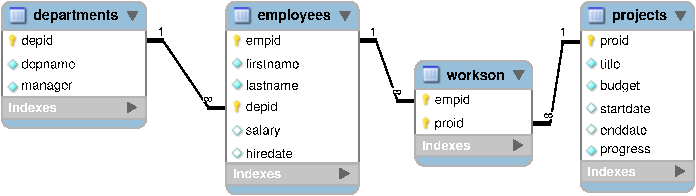
\includegraphics[scale=0.9]{../common/companyREL.pdf}
\vspace{0.5cm}
\begin{itemize} \itemsep 6pt
  \item {\ra departments}, τα τμήματα της εταιρείας.
  \item {\ra employees}, οι υπάλληλοι της εταιρείας.
  \item {\ra projects}, τα έργα που εκτελεί η εταιρεία.
  \item {\ra workson}, η απασχόληση των υπαλλήλων στα έργα.
\end{itemize}
\end{minipage}
\end{frame}


\section[]{\textgreek{Πλήθος υπαλλήλων ανά τμήμα με μισθό άνω των 1300 \euro}}

\begin{frame}[t, fragile, shrink]
\frametitle{Ομαδοποίηση 1:Ν }
\begin{minipage}{\wE}
\begin{block}{\small Να βρεθεί το πλήθος των εργαζομένων με μισθό μεγαλύτερο των 1300 \euro\ ανά όνομα τμήματος}
\pause
\en
\begin{SQL}
 depname                          COUNT(*)
------------------------------------------
&mgr{ Γραμματείας              }               1
&mgr{ Διοίκησης/Επίβλεψης      }               3
&mgr{ Εξωτερικών συνεργατών    }               1
&mgr{ Επιστημόνων/Μηχανικών    }               3
&mgr{ Μάνατζμεντ/Πωλήσεων      }               5
&mgr{ Οικονομoλόγων/Λογιστών   }               3
\end{SQL}
\el
\pause
\begin{itemize}
  \item Δεδομένα από δύο πίνακες: {\ra departments, employees},
        επομένως θα χρειαστεί κάποιου είδους σύζευξη.
  \item Ομαδοποίηση απαραίτητη: {\bb πλήθος ανά ...}
\end{itemize}
\end{block}
\end{minipage}
\end{frame}


\begin{frame}[fragile]
\frametitle{Έχουμε ξαναδεί παρόμοιο παράδειγμα}
\begin{minipage}{\wE}
\begin{exampleblock}{\small Πλήθος υπαλλήλων  ανά τμήμα}
\[ {}_{depid} \mathcal{G}_{count(*)} (employees) \]
\pause
\vspace{-0.5cm}
\begin{columns}[T]
\begin{column}{0.5\textwidth}
\en
\begin{SQL}
  SELECT depid, COUNT(*)
    FROM employees
GROUP BY depid;
\end{SQL}
\el
\end{column}
\begin{column}{0.4\textwidth}
\begin{tabular}{r r} \toprule
{\en \bf depid} & {\en \bf COUNT(*)}\\ \midrule
     1    &     3 \\
     2    &     4 \\
     3    &     9 \\
     4    &     5 \\
     5    &     2 \\
     6    &     7 \\ \hline
\end{tabular}
\el
\end{column}
\end{columns}
\end{exampleblock}
\end{minipage}
\end{frame}

\begin{frame}[t, fragile, shrink]
\frametitle{Ομαδοποίηση 1:Ν -- βήμα 1}
\begin{minipage}{\wE}
  \begin{block}{Τρόπος σκέψης}
    \par Χρειαζόμαστε το όνομα τμήματος, δηλαδή το πεδίο {\ra depname} του πίνακα {\ra departments}.
    \par Οι υπάλληλοι αποθηκεύονται στον πίνακα {\ra employees},
και γνωρίζουμε ότι το πεδίο {\ra depid} του πίνακα αυτού μας πληροφορεί
για το τμήμα όπου απασχολείται κάθε υπάλληλος. 
  \end{block}
  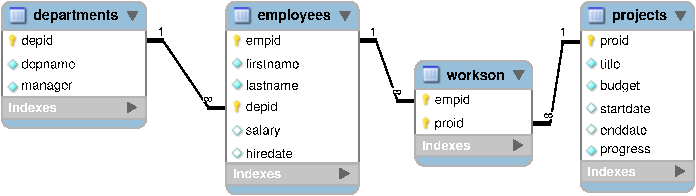
\includegraphics[scale=0.9]{../common/companyREL.pdf}
\end{minipage}
\end{frame}


\begin{frame}[t, fragile, shrink]
\frametitle{Ομαδοποίηση 1:Ν -- βήμα 2}
\begin{minipage}{\wE}
Οι πίνακες {\ra departments} και {\ra employees} έχουν συσχέτιση ένα προς πολλά,
το πεδίο {\ra employees.depid} είναι {\cee ξένο κλειδί}.
\pause
\begin{block}{Σύνδεση πινάκων:}
\[
  departments  \bowtie_{departments.depid  = employees.depid} employees
\]
\vspace*{-1em}
\en
\begin{SQL}
    FROM departments  INNER JOIN employees
         ON departments.depid  = employees.depid
\end{SQL}
\el
\end{block}
\pause
\begin{block}{ή με τη χρήση ψευδωνύμων των πινάκων:}
\[
   \varrho_{d}(departments)  \bowtie_{d.depid = e.depid}  \varrho_{e}(employees)
\]
\vspace*{-1em}
\en
\begin{SQL}
    FROM employees e INNER JOIN departments d
                     ON e.depid = d.depid
\end{SQL}
\el
\end{block}
\end{minipage}
\end{frame}



\begin{frame}[t, fragile, shrink]
\frametitle{Ομαδοποίηση 1:Ν -- βήμα 3}
\begin{minipage}{\wE}
  \begin{block}{Περιορισμός εγγραφών}
Υπάρχει ο περιορισμός για τον μισθό των υπαλλήλων στο ερώτημα.
Επομένως πρέπει να συμπληρωθεί ο όρος \twhere:
\[
   \sigma_{e.salary > 1300}
   (
     \varrho_{d}(departments)  \bowtie_{d.depid = e.depid}  \varrho_{e}(employees)
   )
\]
\pause
\en
\begin{SQL}
    FROM employees e INNER JOIN departments d
         ON e.depid = d.depid
   WHERE e.salary > 1300
\end{SQL}
\el
  \end{block}
\end{minipage}
\end{frame}



\begin{frame}[t, fragile, shrink]
\frametitle{Ομαδοποίηση 1:Ν -- βήμα 4}
\begin{minipage}{\wE}
  \begin{block}{}
Η φράση {\cbb «ανά τμήμα»} δηλώνει ομαδοποίηση, επομένως χρειαζόμαστε τη συμπλήρωση  όρου {\sq \tgroupby}.
Η ομαδοποίηση χρειάζεται για τον υπολογισμό του πλήθους ({\sq COUNT}) {\cbb «ανά τμήμα»}.

\[
  \begin{split} 
   {}_{d.depname} \calg_{count(*)}
   (
     \sigma_{e.salary > 1300}  \\
     (
       \varrho_{d}(departments)  \bowtie_{d.depid = e.depid}  \varrho_{e}(employees)
     )
   )
  \end{split} 
\]
\pause
\en
\begin{SQL}
    FROM employees e INNER JOIN departments d
         ON e.depid = d.depid
   WHERE e.salary > 1300
GROUP BY d.depname
\end{SQL}
\el
  \end{block}
\end{minipage}
\end{frame}



\begin{frame}[t, fragile, shrink]
\frametitle{Ομαδοποίηση 1:Ν -- βήμα 5}
\begin{minipage}{\wE}
\vspace{-1em}
\begin{block}{Προβολή πεδίων}
Από το σύνολο των πεδίων που διατίθενται μετά τη σύζευξη των πινάκων {\ra employees} και {\ra departments}
μας ζητούνται μόνο το όνομα του τμήματος (άρα {\ra departments.depname})
και το πλήθος εργαζομένων ανά τμήμα, δηλαδή  {\ra COUNT(employees.depid)}:
\[
  \begin{split}
   {}_{d.depname} \calg_{count(*) }
   (
     \sigma_{e.salary > 1300}  \\
     (
       \varrho_{d}(departments)  \bowtie_{d.depid = e.depid}  \varrho_{e}(employees)
     )
   )
  \end{split} 
\]
\pause
\en
\begin{SQL}
  SELECT d.depname, COUNT(e.depid)
    FROM employees e INNER JOIN departments d
         ON e.depid = d.depid
   WHERE e.salary > 1300
GROUP BY d.depname
\end{SQL}
\el
  \end{block}
\end{minipage}
\end{frame}


\begin{frame}[t, fragile, shrink]
\frametitle{Ομαδοποίηση 1:Ν -- βήμα 6}
\begin{minipage}{\wE}
  \begin{block}{Επιπλέον επιλογές και παρατηρήσεις}
     \begin{enumerate} \itemsep 6pt
       \item \pause Δεν υπάρχει κάποια απαίτηση για περιορισμό των εγγραφών
             μετά την ομαδοποίηση, δεν χρειάζεται ο όρος {\sq HAVING}.
       \item \pause  Δεν υπάρχει απαίτηση για ταξινόμηση των εγγραφών του αποτελέσματος,
             δεν χρειάζεται ο όρος {\sq ORDER BY}.
       \item \pause  Το ερώτημα είναι πλήρες λοιπόν.      
    \end{enumerate}
  \end{block}
\end{minipage}
\end{frame}



\begin{frame}[t, fragile, shrink]
\frametitle{Ομαδοποίηση 1:Ν -- Τελική διατύπωση}
\begin{minipage}{\wE}
  \vspace*{-0.6cm}
  \begin{exampleblock}{\small Να βρεθεί το πλήθος των εργαζομένων με μισθό μεγαλύτερο των 1300 \euro\ ανά όνομα τμήματος}
  \pause
  \en
\begin{SQL}
  SELECT d.depname, COUNT(e.depid)
    FROM employees e INNER JOIN departments d
         ON e.depid = d.depid
   WHERE e.salary > 1300
GROUP BY d.depname
 
 depname                          COUNT(*)
------------------------------------------
&mgr{ Γραμματείας              }               1
&mgr{ Διοίκησης/Επίβλεψης      }               3
&mgr{ Εξωτερικών συνεργατών    }               1
&mgr{ Επιστημόνων/Μηχανικών    }               3
&mgr{ Μάνατζμεντ/Πωλήσεων      }               5
&mgr{ Οικονομoλόγων/Λογιστών   }               3
\end{SQL}
\el
\end{exampleblock}
\end{minipage}
\end{frame}


\section[]{\textgreek{Υπάλληλοι σε ακριβώς 2 έργα}}

\begin{frame}[t, fragile, shrink]
\frametitle{Ομαδοποίηση 1:Ν με 3 πίνακες}
\begin{minipage}{\wE}
  \begin{block}{\small Να βρεθούν οι υπάλληλοι (κωδικός, όνομα, όνομα τμήματος)
     που απασχολούνται σε ακριβώς 2 έργα}
\pause \scriptsize
\en
\begin{SQL}

empid  firstname    lastname       depname
------------------------------------------------------
&mgr{  153  Μαρία        Αλεβιζάτου     Οικονομoλόγων/Λογιστών }
&mgr{  234  Αδαμαντία    Θεοτοκάτου     Γραμματείας            }
&mgr{  243  Δέσποινα     Παπαδοπούλου   Οικονομoλόγων/Λογιστών }
&mgr{  431  Κώστας       Παπαδόπουλος   Επιστημόνων/Μηχανικών  }
&mgr{  435  Αντώνης      Παύλου         Επιστημόνων/Μηχανικών  }
&mgr{  483  Ηρακλής      Μανωλάκης      Επιστημόνων/Μηχανικών  }
&mgr{  503  Μαριλένα     Κρέσπα         Οικονομoλόγων/Λογιστών }
&mgr{  835  Αθανάσιος    Πετράκης       Μάνατζμεντ/Πωλήσεων    }
\end{SQL}
\el
\end{block}
\end{minipage}
\end{frame}


\begin{frame}[t, fragile, shrink]
\frametitle{Ομαδοποίηση 1:Ν με 3 πίνακες -- Ανάλυση}
  \vspace*{-1em}
  \begin{block}{\small Ποιοι πίνακες χρειάζονται?}
    \begin{enumerate} 
      \item Στοιχεία υπαλλήλων {\ra empid, firstname, lastname},
            επομένως ο πίνακας {\sq employees}.
      \item Στοιχεία τμήματος {\ra depname},
            επομένως ο πίνακας {\sq departments}.
      \item Στοιχεία απασχόλησης: πλήθος συμμετοχών σε έργα,
            επομένως ο πίνακας {\sq workson}.
      \item Υπενθύμιση: Απασχόληση ενός υπαλλήλου σε 2 έργα σημαίνει πως
            υπάρχουν 2 εγγραφές στον πίνακα {\sq workson} με τον κωδικό του.
    \end{enumerate}
  \end{block}
  \begin{minipage}{\wE}
    \vspace*{6pt}
    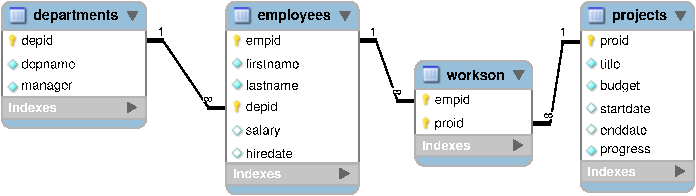
\includegraphics[scale=0.9]{../common/companyREL.pdf}
  \end{minipage}
\end{frame}



\begin{frame}[t, fragile, shrink]
\frametitle{Ομαδοποίηση 1:Ν με 3 πίνακες -- βήμα 1}
\begin{minipage}{\wE}
\vspace{-0.5cm}
  \begin{block}{\small Σύζευξη πινάκων \tdepartments\ και \temployees}
   \[
    \varrho_{d} (departments) \bowtie_{d.depid=e.depid} \varrho_{e} (employees)
   \]
\vspace{-0.5cm}
\en
\begin{SQL}
    FROM departments d INNER JOIN employees e
         ON d.depid = e.depid
\end{SQL}
\el
  \end{block}
  \pause
  \begin{block}{\small Σύζευξη \tdepartments, \temployees\ και \tworkson}
    \[
      \begin{split}
      \varrho_{d} (departments) \bowtie_{d.depid=e.depid} \varrho_{e} (employees)    \\
                                \bowtie_{e.empid=w.empid} \varrho_{w} (workson)     
      \end{split}
    \]
   \vspace{-0.5cm}
\en
\begin{SQL}
    FROM (departments d INNER JOIN employees e
                           ON d.depid = e.depid)
                        INNER JOIN workson w
                           ON e.empid = w.empid
\end{SQL}
\el
  \end{block}
\end{minipage}
\end{frame}



\begin{frame}[t, fragile, shrink]
\frametitle{Ομαδοποίηση 1:Ν με 3 πίνακες -- βήμα 2}
\begin{minipage}{\wE}
\vspace{-0.5cm}
\begin{block}{\small Ομαδοποίηση εγγραφών}
Στο ερώτημα υπάρχει ο περιορισμός για υπαλλήλους που εργάζονται σε 2 ακριβώς έργα.
Απαιτείται η ομαδοποίηση ως προς τα πεδία που ζητούνται στο ερώτημα
{\ra e.empid, e.firstname, e.lastname, d.depname}:
\[
\begin{split}
  {}_{e.empid, e.firstname, e.lastname, d.depname}  \calg_{count(*)} \\
  (
    \varrho_{d} (departments) \bowtie_{d.depid=e.depid} \varrho_{e} (employees) \\
                            \bowtie_{e.empid=w.empid} \varrho_{w} (workson)
  )
\end{split}
\]
\pause
\en
\begin{SQL}
    FROM (departments d INNER JOIN employees e
                           ON d.depid = e.depid)
                        INNER JOIN workson w
                           ON e.empid = w.empid
GROUP BY e.empid, e.firstname, e.lastname, d.depname
\end{SQL}
\el
\end{block}
\end{minipage}
\end{frame}



\begin{frame}[t, fragile, shrink]
\frametitle{Ομαδοποίηση 1:Ν με 3 πίνακες -- βήμα 3}
\begin{minipage}{\wE}
\begin{block}{\small Περιορισμός μετά την ομαδοποίηση}
Είμαστε τώρα σε θέση να εφαρμόσουμε τον περιορισμό
για ακριβώς 2 συμμετοχές υπαλλήλων σε έργα.
Στον όρο {\sq HAVING} και όχι στον όρο {\sq WHERE}:
\[
\begin{split}
  \sigma _{count(*) = 2}
  (
    {}_{e.empid, e.firstname, e.lastname, d.depname}  \calg_{count(*)} \\
    (
      \varrho_{d} (departments) \bowtie_{d.depid=e.depid} \varrho_{e} (employees) \\
                               \bowtie_{e.empid=w.empid} \varrho_{w} (workson)
    )
  )
\end{split}
\]
\pause
\vspace{-0.4cm}
\en
\begin{SQL}
    FROM (departments d INNER JOIN employees e
                           ON d.depid = e.depid)
                        INNER JOIN workson w
                           ON e.empid = w.empid
GROUP BY e.empid, e.firstname, e.lastname, d.depname
  HAVING COUNT(*) = 2
\end{SQL}
\el
  \end{block}
\end{minipage}
\end{frame}


\begin{frame}[t, fragile, shrink]
\frametitle{Ομαδοποίηση 1:Ν με 3 πίνακες -- Τελική διατύπωση}
\begin{minipage}{\wE}
\vspace{-0.5cm}
\begin{block}{\small Τελική διατύπωση: υπάλληλοι σε 2 έργα}
\[
\begin{split}
  \Pi_{e.empid, e.firstname, e.lastname, d.depname}  \\
  (
    \sigma _{count(*) = 2}
    (
      {}_{e.empid, e.firstname, e.lastname, d.depname}  \calg_{count(*)} \\
      (
        \varrho_{d} (departments) \bowtie_{d.depid=e.depid} \varrho_{e} (employees) \\
                                  \bowtie_{e.empid=w.empid} \varrho_{w} (workson)
      )
    )
  )
\end{split}
\]
\pause
\en
\begin{SQL}
  SELECT e.empid, e.firstname, e.lastname, d.depname
    FROM (departments d INNER JOIN employees e
                           ON d.depid = e.depid)
                        INNER JOIN workson w
                           ON e.empid = w.empid
GROUP BY e.empid, e.firstname, e.lastname, d.depname
  HAVING COUNT(*) = 2;
\end{SQL}
\el
  \end{block}
\end{minipage}
\end{frame}


\section[]{\textgreek{Έργα με 3 υπαλλήλους του τμήματος 2}}


\begin{frame}[t, fragile, shrink]
\frametitle{Σύζευξη 3 πινάκων, πολλά προς πολλά}
\begin{minipage}{\wE}
\vspace{-0.5cm}
\begin{block}{\small Να βρεθεί ο κωδικός και ο τίτλος των έργων στα οποία απασχολούνται
ακριβώς 3 υπάλληλοι του τμήματος 2}
\pause  
\en
\begin{SQL}
proid   title
--------------------------------------
&mgr{    21  Παροχή συμβουλευτικών υπηρεσιών...}
&mgr{    38  Μελέτη εναλλακτικών λύσεων για...}
\end{SQL}
\el
\end{block}
\pause
\begin{enumerate} \itemsep 4pt
  \item Πληροφορίες από τον πίνακα {\ra projects}
  \item Αναζήτηση με βάση δεδομένα από τους πίνακες {\ra employees, workson}
  \item Λύση: {\crr σύζευξη πινάκων}
  \item Επόμενο μάθημα: {\cee υποερώτημα}
\end{enumerate}
\end{minipage}
\end{frame}



\begin{frame}[t, fragile, shrink]
\frametitle{Πολλά προς πολλά -- πίνακες}
\vspace{-0.5cm}
\begin{block}{Ποιοι πίνακες χρειάζονται?}
    \begin{enumerate}
      \item Στοιχεία έργων {\ra proid, title},
            επομένως ο πίνακας {\sq projects}.
      \item Στοιχεία υπαλλήλων: {\ra depid=2},
            επομένως ο πίνακας {\sq employees}.
      \item Στοιχεία απασχόλησης: πλήθος συμμετοχών σε έργα,
            επομένως ο πίνακας {\sq workson}.
      \item Υπενθύμιση: Απασχόληση ενός υπαλλήλου σε 3 έργα σημαίνει πως
            υπάρχουν 2 εγγραφές στον πίνακα {\sq workson} με τον κωδικό του.
    \end{enumerate}
\end{block}
\begin{minipage}{\wE}
  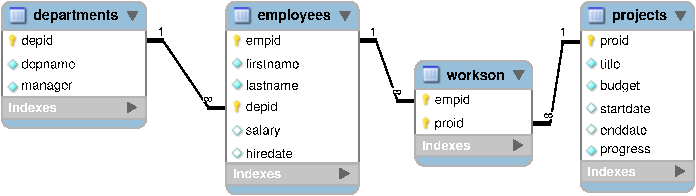
\includegraphics[scale=0.9]{../common/companyREL.pdf}  
\end{minipage}  
\end{frame}



\begin{frame}[t, fragile, shrink]
\frametitle{Πολλά προς πολλά -- βήμα 1}
\begin{minipage}{\wE}
\vspace{-0.5cm}
\begin{block}{\small Σύζευξη {\en\em employees, workson, projects}}
\[
  \begin{split}
      \varrho_{e} (employees) \bowtie_{e.empid=w.empid} \varrho_{w} (workson)  \\
                              \bowtie_{w.proid=p.proid} \varrho_{p} (projects)
  \end{split}
\]
\vspace*{-1em}
\pause
\en
\begin{SQL}
    FROM (employees e INNER JOIN workson w
                         ON e.empid = w.empid)
                      INNER JOIN projects p
                         ON w.proid = p.proid
\end{SQL}
\el  
\end{block}
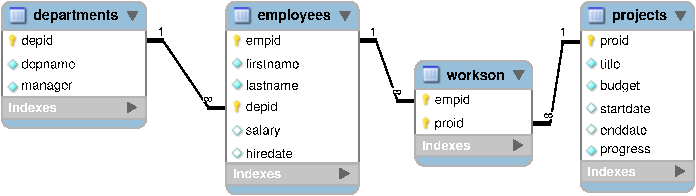
\includegraphics[scale=0.9]{../common/companyREL.pdf}
\end{minipage}
\end{frame}


\begin{frame}[t, fragile, shrink]
\frametitle{Πολλά προς πολλά -- βήμα 2}
\begin{minipage}{\wE}
\vspace{-0.5cm}
\begin{block}{Περιορισμός εγγραφών {\en e.depid=2}}
Υπάρχει o περιορισμός που αφορά τους υπαλλήλους του τμήματος 2:
\[
\begin{split}
    \sigma_{e.depid=2}
    (                           \\
      \varrho_{e} (employees) \bowtie_{e.empid=w.empid} \varrho_{w} (workson)  \\
                              \bowtie_{w.proid=p.proid} \varrho_{p} (projects)
    )
\end{split}
\]
\vspace{-0.5cm}
\pause
\en
\begin{SQL}
    FROM (employees e INNER JOIN workson w
                         ON e.empid = w.empid)
                      INNER JOIN projects p
                         ON w.proid = p.proid
   WHERE e.depid = 2
\end{SQL}
\el
  \end{block}
\end{minipage}
\end{frame}


\begin{frame}[t, fragile, shrink]
\frametitle{Πολλά προς πολλά -- βήμα 3}
\begin{minipage}{\wE}
\vspace{-0.5cm}
\begin{block}{\small Ομαδοποίηση εγγραφών}
Στο ερώτημα υπάρχει ο περιορισμός για ακριβώς 3 συμμετοχές υπαλλήλων σε έργα.
Απαιτείται η εφαρμογή ομαδοποίησης εγγραφών ως προς τα ζητούμενα του ερωτήματος:
\pause
\[
\begin{split}
  {}_{p.proid, p.title} \calg_{count(*)}
    (
      \sigma_{e.depid=2}
      (                           \\
        \varrho_{e} (employees) \bowtie_{e.empid=w.empid} \varrho_{w} (workson)  \\
                                \bowtie_{w.proid=p.proid} \varrho_{p} (projects)
      )
    )
\end{split}
\]
\pause
\vspace{-0.5cm}
\en
\begin{SQL}
    FROM (employees e INNER JOIN workson w
                         ON e.empid = w.empid)
                      INNER JOIN projects p
                         ON w.proid = p.proid
   WHERE e.depid = 2
GROUP BY p.proid, p.title
\end{SQL}
\el
  \end{block}
\end{minipage}
\end{frame}


\begin{frame}[t, fragile, shrink]
\frametitle{Πολλά προς πολλά -- βήμα 4}
\begin{minipage}{\wE}
\vspace{-0.5cm}
\begin{block}{\small Περιορισμός μετά την ομαδοποίηση}
Μετά την ομαδοποίηση των εγγραφών
εφαρμόσουμε τον περιορισμό για ακριβώς 3 συμμετοχές των υπαλλήλων στα έργα:
\[
\begin{split}
  \sigma_{count(*)=3}
  (
    {}_{p.proid, p.title} \calg_{count(*)}
    (
      \sigma_{e.depid=2}
      (                           \\
        \varrho_{e} (employees) \bowtie_{e.empid=w.empid} \varrho_{w} (workson)  \\
                                \bowtie_{w.proid=p.proid} \varrho_{p} (projects)
      )
    )
  )
\end{split}
\]
\pause
\vspace{-0.5cm}
\en
\begin{SQL}
    FROM (employees e INNER JOIN workson w
                         ON e.empid = w.empid)
                      INNER JOIN projects p
                         ON w.proid = p.proid
   WHERE e.depid = 2
GROUP BY p.proid, p.title
  HAVING COUNT(*) = 3
\end{SQL}
\el
  \end{block}
\end{minipage}
\end{frame}


\begin{frame}[t, fragile, shrink]
\frametitle{Πολλά προς πολλά -- Τελική διατύπωση}
\begin{minipage}{\wE}
\vspace{-0.5cm}
\begin{block}{\small Ποια πεδία θέλουμε στο αποτέλεσμα:}
\[
\begin{split}
  \Pi_{p.proid, p.title}
  (
    \sigma_{count(*)=3}
    (
      {}_{p.proid, p.title} \calg_{count(*)}
      (
        \sigma_{e.depid=2}
        (                           \\
          \varrho_{e} (employees) \bowtie_{e.empid=w.empid} \varrho_{w} (workson)  \\
                                  \bowtie_{w.proid=p.proid} \varrho_{p} (projects)
        )
      )
    )
  )
\end{split}
\]
\pause
\vspace{-0.5cm}
\en
\begin{SQL}
  SELECT p.proid, p.title
    FROM (employees e INNER JOIN workson  w
                         ON e.empid = w.empid)
                      INNER JOIN projects p
                         ON p.proid = w.proid
   WHERE e.depid = 2
GROUP BY p.proid, p.title
  HAVING COUNT(*) = 3;
\end{SQL}
\el
\end{block}
\end{minipage}
\end{frame}




\section[]{\textgreek{Απασχόληση σε έργα των υπαλλήλων του τμήματος 4}}


\begin{frame}[t, fragile, shrink]
\frametitle{Πλήθος υπαλλήλων ανά έργο}
\begin{minipage}{\wE}
\vspace{-0.5cm}
\begin{block}{\small Να βρεθεί το πλήθος των των συμμετοχών σε έργα των υπαλλήλων του τμήματος 4,
ανά κωδικό και τίτλο έργου στα οποία απασχολούνται}
\pause
\en
\begin{SQL}
 proid  title                           COUNT(*)
------------------------------------------------
&mgr{    12  Επίβλεψη κατασκευής σταθμού...         2}
&mgr{    14  Μελέτη και επίβλεψη κατασκευής...      1}
&mgr{    38  Μελέτη εναλλακτικών λύσεων για...      1}
&mgr{    43  Μελέτη οικονομικής βιωσιμότητας...     1}
\end{SQL}
\el
\end{block}
\pause
\begin{enumerate}
  \item Πληροφορίες από τον πίνακα {\ra projects}
  \item Αναζήτηση με βάση δεδομένα από τους πίνακες {\ra employees, workson}
  \item Λύση: {\crr σύζευξη πινάκων}
\end{enumerate}
\end{minipage}
\end{frame}



\begin{frame}[t, fragile, shrink]
\frametitle{Πλήθος υπαλλήλων ανά έργο}
\vspace{-0.5cm}
  \begin{block}{\small Ποιοι πίνακες χρειάζονται?}
    \begin{enumerate} \itemsep 4pt
      \item Στοιχεία έργων {\ra proid, title}, επομένως ο πίνακας {\sq projects}.
      \item Στοιχεία υπαλλήλων: {\ra depid=4}, επομένως ο πίνακας {\sq employees}.
      \item Στοιχεία απασχόλησης: πλήθος συμμετοχών σε έργα, επομένως ο πίνακας {\sq workson}.
    \end{enumerate}
  \end{block}
\begin{minipage}{\wE}
  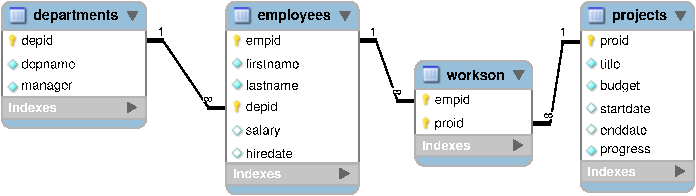
\includegraphics[scale=0.9]{../common/companyREL.pdf}
\end{minipage}
\end{frame}



\begin{frame}[t, fragile, shrink]
\frametitle{Πλήθος υπαλλήλων ανά έργο -- βήμα 1}
\begin{minipage}{\wE}
\vspace{-0.5cm}
\begin{block}{\small Σύζευξη πινάκων}
\[
  \begin{split}
      \varrho_{e} (employees) \bowtie_{e.empid=w.empid} \varrho_{w} (workson)  \\
                              \bowtie_{w.proid=p.proid} \varrho_{p} (projects)
  \end{split}
\]
\vspace{-0.5cm}
\pause
\en
\begin{SQL}
    FROM (employees e INNER JOIN workson w
                         ON e.empid = w.empid)
                      INNER JOIN projects p
                         ON w.proid = p.proid
\end{SQL}
\el
\end{block}
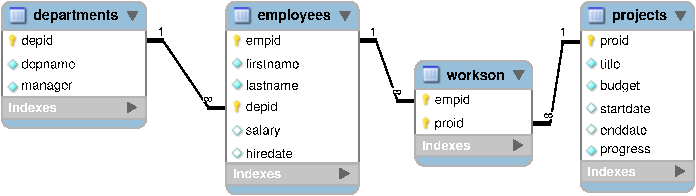
\includegraphics[scale=0.9]{../common/companyREL.pdf}
\end{minipage}
\end{frame}


\begin{frame}[t, fragile, shrink]
\frametitle{Πλήθος υπαλλήλων ανά έργο -- βήμα 2}
\begin{minipage}{\wE}
\vspace{-0.5cm}
\begin{block}{\small Περιορισμός εγγραφών {\en e.depid=4}}
Υπάρχει o περιορισμός που αφορά τους υπαλλήλους του τμήματος 4:
\[
\begin{split}
    \sigma_{e.depid=4}
    (                           \\
      \varrho_{e} (employees) \bowtie_{e.empid=w.empid} \varrho_{w} (workson)  \\
                              \bowtie_{w.proid=p.proid} \varrho_{p} (projects)
    )
\end{split}
\]
\vspace*{-1em}
\pause
\en
\begin{SQL}
    FROM (employees e INNER JOIN workson w
                         ON e.empid = w.empid)
                      INNER JOIN projects p
                         ON w.proid = p.proid
   WHERE e.depid = 4
\end{SQL}
\el
\end{block}
\end{minipage}
\end{frame}


\begin{frame}[t, fragile, shrink]
\frametitle{Πλήθος υπαλλήλων ανά έργο -- βήμα 3}
\begin{minipage}{\wE}
\vspace{-0.5cm}
\begin{block}{\small Ομαδοποίηση}
  «πλήθος των υπαλλήλων ανά έργο», δηλαδή {\crr ομαδοποίηση}:\\
\[
\begin{split}
  {}_{p.proid, p.title} \calg_{count(*)}
    (
      \sigma_{e.depid=4}
      (                           \\
        \varrho_{e} (employees) \bowtie_{e.empid=w.empid} \varrho_{w} (workson) \\
                                \bowtie_{w.proid=p.proid} \varrho_{p} (projects)
      )
    )
\end{split}
\]
\pause
\en
\begin{SQL}
    FROM (employees e INNER JOIN workson w
                         ON e.empid = w.empid)
                      INNER JOIN projects p
                         ON w.proid = p.proid
   WHERE e.depid = 4
GROUP BY p.proid, p.title
\end{SQL}
\el
\end{block}
\end{minipage}
\end{frame}


\begin{frame}[t, fragile, shrink]
\frametitle{Πλήθος υπαλλήλων ανά έργο -- βήμα 4}
\begin{minipage}{\wE}
\vspace{-0.5cm}
\begin{block}{\small Τελική διατύπωση}
\[
\begin{split}
      {}_{p.proid, p.title} \calg_{count(*)}
      (
        \sigma_{e.depid=2}
        (                           \\
          \varrho_{e} (employees) \bowtie_{e.empid=w.empid} \varrho_{w} (workson) \\
                                  \bowtie_{w.proid=p.proid} \varrho_{p} (projects)
        )
      )
\end{split}
\]
\pause
\en
\begin{SQL}
  SELECT p.proid, p.title, COUNT(*)
    FROM (employees e INNER JOIN workson  w
                         ON e.empid = w.empid)
                      INNER JOIN projects p
                         ON p.proid = w.proid
   WHERE e.depid = 4
GROUP BY p.proid, p.title;
\end{SQL}
\el
\end{block}
\end{minipage}
\end{frame}




\section[]{\textgreek{Πλήθος υπαλλήλων που προσλήφθηκαν το 2002 και εργάζονται σε έργα με πρόοδο $<75\%$}}


\begin{frame}[t, fragile, shrink]
\frametitle{Πρόσληψη το 2002}
\begin{block}{\small Να βρεθεί το πλήθος των υπαλλήλων που προσλήφθηκαν
μέσα στο 2002 και απασχολούνται σε έργα με βαθμό προόδου μικρότερο του 75\%}
\pause
\en
\begin{SQL}
 COUNT(DISTINCT e.empid)
------------------------
                       3
\end{SQL}
\el
\end{block}
\pause
\vspace{0.5cm}
\begin{minipage}{\wE}
\begin{enumerate} \itemsep 4pt
  \item Πληροφορίες από τον πίνακα {\ra employees}
  \item Αναζήτηση με βάση δεδομένα από τους πίνακες {\ra employees, projects}
  \item Λύση: {\crr σύζευξη πινάκων}
  \item {\crr Προσοχή} στη χρήση του πίνακα {\ra workson}
\end{enumerate}
\end{minipage}
\end{frame}


\begin{frame}[t, fragile, shrink]
\frametitle{Πρόσληψη το 2002 και πρόοδος έργων}
\begin{minipage}{\wE}
  \vspace{-0.5cm}
  \begin{block}{Ποιοι πίνακες χρειάζονται?}
    \begin{enumerate} \itemsep 6pt
      \item Στοιχεία υπαλλήλων {\ra empid, hiredate}, επομένως ο πίνακας {\sq employees}.
      \item Στοιχεία έργων: {\ra progress}, επομένως ο πίνακας {\sq projects}.
      \item Σύζευξη πινάκων υπαλλήλων και έργων, επομένως ο πίνακας {\sq workson}.
    \end{enumerate}
  \end{block}
  \vspace{0.5cm}
  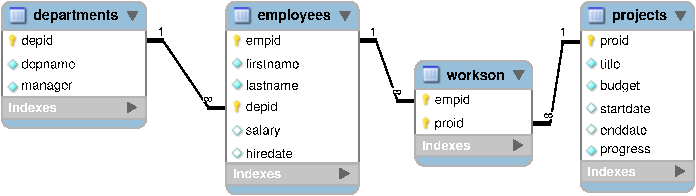
\includegraphics[scale=0.9]{../common/companyREL.pdf}
\end{minipage}
\end{frame}



\begin{frame}[t, fragile, shrink]
\frametitle{Πρόσληψη το 2002 -- βήμα 1}
\begin{minipage}{\wE}
\vspace{-0.5cm}
\begin{block}{\small Σύζευξη πινάκων}
\[
  \begin{split}
      \varrho_{e} (employees) \bowtie_{e.empid=w.empid} \varrho_{w} (workson)  \\
                              \bowtie_{w.proid=p.proid} \varrho_{p} (projects)
  \end{split}
\]
\vspace{-0.5cm}
\pause
\en
\begin{SQL}
    FROM (employees e INNER JOIN workson  w
                         ON e.empid = w.empid)
                      INNER JOIN projects p
                         ON w.proid = p.proid
\end{SQL}
\el
\end{block}
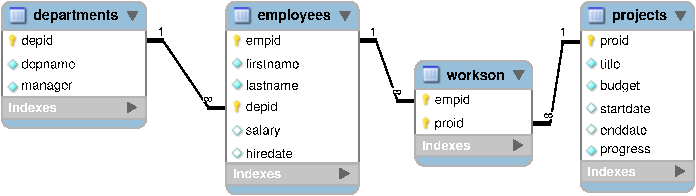
\includegraphics[scale=0.9]{../common/companyREL.pdf}
\end{minipage}
\end{frame}



\begin{frame}[t, fragile, shrink]
\frametitle{Πρόσληψη το 2002 -- βήμα 2}
\begin{minipage}{\wE}
\vspace{-0.5cm}
  \begin{block}{\small Περιορισμός εγγραφών }
Περιορισμός με βάση την ημερομηνία πρόσληψης και την πρόοδο έργου:
\[
\begin{split}
      \sigma_{\sigma_{e.hiredate\geq'2002-01-01'\wedge e.hiredate\leq'2002-12-31'}
                      \wedge p.progress>75}
      (                           \\
        \varrho_{e} (employees) \bowtie_{e.empid=w.empid} \varrho_{w} (workson) \\
                                \bowtie_{w.proid=p.proid} \varrho_{p} (projects)
      )
\end{split}
\]
\pause
\vspace{-0.5cm}
\en
\begin{SQL}
    FROM (employees e INNER JOIN workson  w
                         ON e.empid = w.empid)
                      INNER JOIN projects p
                         ON w.proid = p.proid
   WHERE e.hiredate BETWEEN '2002-01-01' AND '2002-12-31'
     AND p.progress < 75
\end{SQL}
\el
\end{block}
\end{minipage}
\end{frame}



\begin{frame}[t, fragile, shrink]
\frametitle{Πρόσληψη το 2002 -- τελική διατύπωση}
\begin{minipage}{\wE}
\vspace{-0.55cm}
  \begin{block}{\small Καταμέτρηση πλήθους}
\[
\begin{split}
    {}_{} \calg_{count(e.empid)}    
      \sigma_{\sigma_{e.hiredate\geq'2002-01-01'\wedge e.hiredate\leq'2002-12-31'}
                      \wedge p.progress>75}
      (                           \\
        \varrho_{e} (employees) \bowtie_{e.empid=w.empid} \varrho_{w} (workson)   \\
                                \bowtie_{w.proid=p.proid} \varrho_{p} (projects)
      )
\end{split}
\]
\pause
\vspace{-0.55cm}
\en
\begin{SQL}
  SELECT COUNT(DISTINCT e.empid)
    FROM (employees e INNER JOIN workson  w
                         ON e.empid = w.empid)
                      INNER JOIN projects p
                         ON p.proid = w.proid
   WHERE e.hiredate BETWEEN '2002-01-01' AND '2002-12-31'
     AND p.progress < 75;

 COUNT(DISTINCT e.empid)
------------------------
                       3
\end{SQL}
\el
\end{block}
\end{minipage}
\end{frame}


\begin{frame}[t, fragile, shrink]
\frametitle{Πρόσληψη το 2002 -- λάθος διατύπωση}
\begin{minipage}{\wE}
\vspace{-0.55cm}
\begin{alertblock}{\small Χωρίς απαλοιφή διπλοεγγραφών}
\vspace{-0.55cm}
\[
\begin{split}
    {}_{} \calg_{count(e.empid)}
      \sigma_{\sigma_{e.hiredate\geq'2002-01-01'\wedge e.hiredate\leq'2002-12-31'}
                      \wedge p.progress>75}
      (                           \\
        \varrho_{e} (employees) \bowtie_{e.empid=w.empid} \varrho_{w} (workson)   \\
                                \bowtie_{w.proid=p.proid} \varrho_{p} (projects)
      )
\end{split}
\]
\pause
\vspace{-0.55cm}
\en
\begin{SQL}
  SELECT &color{red}COUNT(e.empid) &color{black}
    FROM (employees e INNER JOIN workson  w
                         ON e.empid = w.empid)
                      INNER JOIN projects p
                         ON p.proid = w.proid
   WHERE e.hiredate BETWEEN '2002-01-01' AND '2002-12-31'
     AND p.progress < 75;

 COUNT(e.empid)
---------------
              5
\end{SQL}
\el
\end{alertblock}
\end{minipage}
\end{frame}


\begin{frame}[t, fragile, shrink]
\frametitle{Πρόσληψη το 2002 -- γιατί {\en DISTINCT}?}
\begin{minipage}{\wE}
\vspace{-0.55cm}
\begin{block}{\small Τι παρατηρείτε?}
\en
\begin{SQL}
  SELECT e.empid, e.hiredate, p.proid, p.progress
    FROM (employees e INNER JOIN workson  w
                         ON e.empid = w.empid)
                      INNER JOIN projects p
                         ON w.proid = p.proid
   WHERE e.hiredate BETWEEN '2002-01-01' AND '2002-12-31'
     AND p.progress < 75;

 empid  hiredate    proid  progress
------------------------------------
   206  2002-12-03     12      60.0
   230  2002-12-03     12      60.0
   230  2002-12-03     14      20.0
   431  2002-09-16     14      20.0
   230  2002-12-03     38       0.0
\end{SQL}
\el
\end{block}
\end{minipage}
\end{frame}


\begin{frame}[t, fragile, shrink]
\frametitle{Διαχωρισμός δύο εννοιών}
\begin{minipage}{\wE}
\pause
\vspace{-0.7cm}
\begin{alertblock}{\small Πλήθος συμμετοχών υπαλλήλων σε έργα}
\en
\begin{SQL}
  SELECT COUNT(e.empid)
    FROM (employees e INNER JOIN workson  w
                         ON e.empid = w.empid)
                      INNER JOIN projects p
                         ON w.proid = p.proid
   WHERE e.hiredate BETWEEN '2002-01-01' AND '2002-12-31'
     AND p.progress < 75;
\end{SQL}
\el
\end{alertblock}
\pause
\vspace{-0.7cm}
\begin{exampleblock}{\small Πλήθος υπαλλήλων που απασχολούνται σε έργα}
\en
\begin{SQL}
  SELECT COUNT(DISTINCT e.empid)
    FROM (employees e INNER JOIN workson  w
                         ON e.empid = w.empid)
                      INNER JOIN projects p
                         ON w.proid = p.proid
   WHERE e.hiredate BETWEEN '2002-01-01' AND '2002-12-31'
     AND p.progress < 75;
\end{SQL}
\el
\end{exampleblock}  
\end{minipage}
\end{frame}



\section[]{\textgreek{Ασκήσεις επανάληψης}}

% 8
\begin{frame}[t, fragile, shrink]
\frametitle{Πλήθος υπαλλήλων ανά έργο ...}
\begin{minipage}{\wE}
\vspace{-0.5cm}
\begin{exampleblock}{\small Να βρεθεί το πλήθος των εργαζομένων με μισθό
        μικρότερο του 1500, ανά κωδικό και τίτλο έργου,
        με αύξουσα ταξινόμηση ως προς το πλήθος εργαζομένων,
        για έργα που απασχολούν λιγότερο 
        από 5 υπαλλήλους.}
\pause
\en
\begin{SQL}
  SELECT p.proid, p.title, COUNT(*)
    FROM (employees e INNER JOIN workson  w
                         ON e.empid = w.empid)
                      INNER JOIN projects p
                         ON p.proid = w.proid    &pause
   WHERE e.salary < 1500   &pause
GROUP BY p.proid, p.title  &pause
  HAVING COUNT(*) < 5      &pause
ORDER BY COUNT(*) ASC;      
\end{SQL}
\end{exampleblock}
\end{minipage}
\end{frame}


% 13
\begin{frame}[t, fragile, shrink]
\frametitle{Μισθοδοσία ανά τμήμα ...}
\begin{minipage}{\wE}
\vspace{-0.5cm}
\begin{exampleblock}{\small Να βρεθεί ο κωδικός και το όνομα των τμημάτων, καθώς και το άθροισμα μισθοδοσίας
        των υπαλλήλων ανά τμήμα, που απασχολούνται σε όλα τα έργα με πρόοδο πάνω
        από 50\%, και που απασχολούν (τα έργα) περισσότερους από
        έναν υπαλλήλους.}
\pause
\en
\begin{SQL}
  SELECT d.depid, d.depname, SUM(DISTINCT e.salary)
    FROM ((employees e INNER JOIN departments d
                          ON e.depid = d.depid)
                       INNER JOIN workson  w
                          ON e.empid = w.empid)
                       INNER JOIN projects p
                          ON p.proid = w.proid   &pause
   WHERE p.progress > 50          &pause
GROUP BY d.depid, d.depname       &pause
  HAVING COUNT(*) > 1;   
\end{SQL}
\end{exampleblock}
\end{minipage}
\end{frame}


% 14
\begin{frame}[fragile, shrink]
\frametitle{Διευθυντές και έργα}
\begin{minipage}{\wE}
\begin{exampleblock}{\small Να βρεθεί το όνομα του τμήματος,
            το επώνυμο και ο κωδικός του διευθυντή και το πλήθος
            των έργων στα οποία απασχολείται ο κάθε διευθυντής.}
\pause
\en
\begin{SQL}
 SELECT d.depname, e.lastname, w.empid, COUNT(*)
   FROM  (departments d INNER JOIN employees e
                           ON d.manager = e.empid)
                         LEFT JOIN workson w
                           ON e.empid = w.empid  
GROUP BY d.depname, e.lastname, w.empid;
\end{SQL}
\end{exampleblock}
\vspace{0.2cm}
\begin{enumerate}
  \item Σχολιάστε την ύπαρξη της αριστερής σύζευξης.
        Είναι προαιρετική ή απαραίτητη?
  \item Θα έχει νόημα να ήταν αριστερή σύζευξη
        η σύζευξη ανάμεσα σε {\ra departments} και {\ra employees}?
\end{enumerate}

\end{minipage}
\end{frame}





\begin{frame}
\frametitle{Σχόλια και ερωτήσεις}
\par {\Huge \color{red} Σας ευχαριστώ \\ για την προσοχή σας }
\vspace{1cm}
\par Είμαι στη διάθεσή σας για σχόλια, απορίες και ερωτήσεις
\end{frame}

\end{document}





\begin{frame}[t, fragile, shrink]
\frametitle{Πρόσληψη το 2002 -- βήμα 1}
\begin{minipage}{0.94\textwidth}
  \vspace*{-1em}
  \begin{block}{Ομαδοποίηση}

  \end{block}
\end{minipage}
\end{frame}
